\begin{center}
  \textbf{Базис(ИЛИ-НЕ)}
\end{center}

Приведение аналитического выражения (2) к базису (ИЛИ-НЕ) осуществляется заменой операций булева базиса на операцию стрелка Пирса (отрицание дизъюнкции) путем использования законов двойственности. 

$
\phi = \nx{2}\nx{3}= \overline{\overline{\nx{2}\nx{3}}}= \overline{\pirs{\nx{2}}{\nx{3}}} \rightarrow \nphi = \pirs{\nx{2}}{\nx{3}} 
$

\begin{align*}
f &= (\x{1}\vee\x{3}\vee\nx{2}\x{4})(\nx{1}\vee(\x{5}\vee\x{4}\nphi)(\nx{3} \vee \nx{4} \vee \phi)) = \\
  &=\neg{ \x{1}\vee\x{3}\vee \neg{\x{2}\vee\nx{4}} }
    \vee
    \neg{
      \nx{1} \vee
      \neg{ \x{5} \vee \neg{\nx{4}\vee\phi}} \vee
      \neg{ \nx{3} \vee \nx{4} \vee \phi   }
    } = \\
  &=(\x{1}\downarrow\x{3}\downarrow (\x{2}\downarrow\nx{4}))
    \downarrow
    (\nx{1} \downarrow
      (
        (\x{5} \downarrow (\nx{4}\downarrow\phi)) 
        \downarrow
        (\nx{3} \downarrow \nx{4} \downarrow \phi)
      )
    )
\end{align*}

По полученному выражению строим схему с парафазными входами в базисе (ИЛИ-НЕ):
\begin{center}
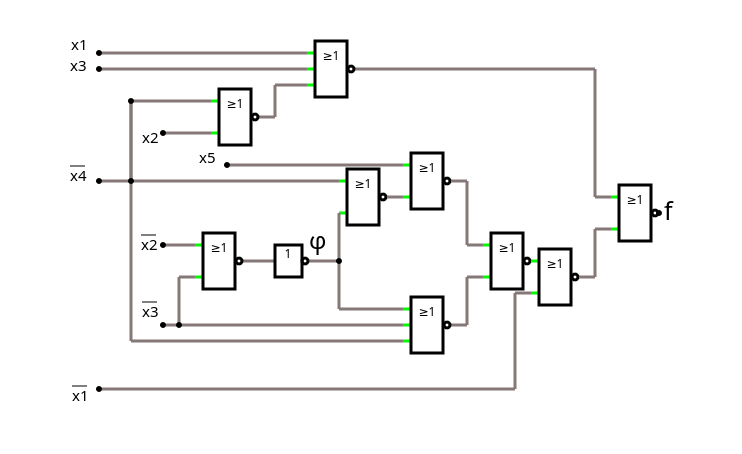
\includegraphics[width=\linewidth]{imgs/circuit-ORNOT_basis.png}
\end{center}
Задержка схемы $Т=7\tau$, цена схемы $S_Q=21$. По сравнению с ценой схемы $S_Q$, определенной по выражению (2), цена построенной схемы не изменилась. 
% ---------

\begin{center}
  \textbf{Базис(И-НЕ)}
\end{center}
Приведение аналитического выражения (2) к базису (И-НЕ) осуществляется заменой операций булева базиса на операцию штрих Шеффера (отрицание конъюнкции) путем использования законов двойственности.

$
\phi = \nx{2}\nx{3} = \overline{\nx{2}|\nx{3}} \rightarrow \nphi = \nx{2}|\nx{3} 
$

\begin{align*}
f &= (\x{1}\vee\x{3}\vee\nx{2}\x{4})(\nx{1}\vee(\x{5}\vee\x{4}\nphi)(\nx{3} \vee \nx{4} \vee \phi)) = \\
  &=\neg{\nx{1}\nx{3} \neg{\nx{2}\cdot\x{4}}} \cdot
    \neg{
      \x{1} 
      \neg{ \nx{5} \neg{\x{4}\cdot\nphi}} \cdot
      \neg{ \x{3}\x{4}\nphi}
    } = \\
\
  &=\neg{(\nx{1}|\nx{3}|(\nx{2}|\x{4})) |
  (
    \x{1} |
    (\nx{5}|(\x{4}|\nphi)) |
    (\x{3}|\x{4}|\nphi)
  )}
\end{align*}

\begin{center}
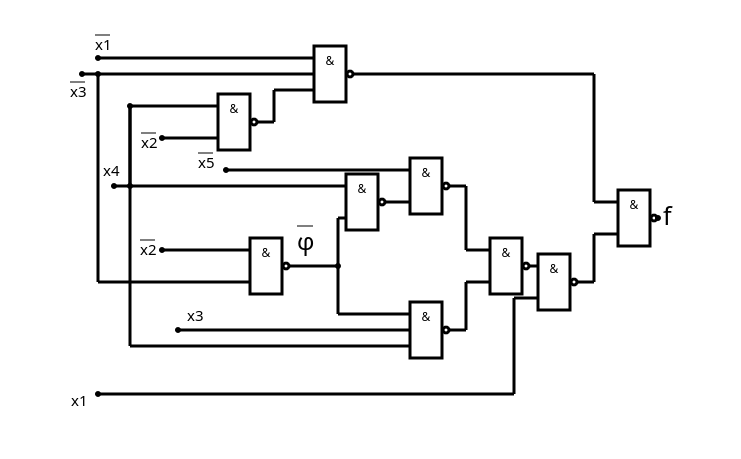
\includegraphics[width=\linewidth]{imgs/circuit-ANDNOT_basis.png}
\end{center}
Задержка схемы $Т=6\tau$, цена схемы $S_Q=20$.